
Google Docs made real-time editing in browsers easy for millions of
users. However, Google mediates real-time editing sessions with central servers
raising issues on privacy, censorship, economic intelligence. It also raises
scalability issues in term of number of participants.  Despite that small groups
currently constitute the main range of users, events such as massive online
lectures, TV shows, conferences gather larger groups.  Google Docs supports
large groups but only the first fifty users can edit, next users have their
rights limited to document reading. We think that real-time editors should allow
editing at anytime and anywhere, whatever the number of participants.  Real-time
editing sessions can be highly dynamic; even if only few authors are editing a
document simultaneously, the editing session includes a much larger group of
potential writers.

%% In this paper we focus on building a real-time editor that supports privacy
%% and that adapts \TODO{gently} from small groups to large groups

Decentralized real-time editors~\cite{oster2006data, sun1998operational,
  sun2009contextbased} do not require intermediate servers and by the same
settle privacy issues. However, scalability issues remain.  Addressing
scalability requires finding a good trade-off between communication, space and
time complexities. Achieving a sublinear communication complexity compared to
the editing session size is crucial for supporting large groups.

%% But consistency maintenance of documents requires each message to piggyback
%% additional information which greatly impacts the communication complexity.

To provide availability and responsiveness of documents, real-time editors use
the optimistic replication. As such, each user creates a local copy of the
document and directly performs her modification on it. Changes are broadcast to
all replica owners where they are integrated. Strong eventual consistency states
that replicas integrating an identical set of operations converge to an
equivalent state, i.e., users read a same document.

Decentralized algorithms of operational
transformation~\cite{sun2009contextbased} require piggybacking a state vector in
order to detect concurrent operations. Unfortunately, state vectors grow
linearly compared to the number of members that ever participated in the
authoring. Hence, these approaches behave great in stable environments with
small groups of users but should not be used in large scale system subject to
high latency.

Conflict-Free Replicated Data Types~\cite{shapiro2011comprehensive} (CRDTs)
avoid paying the price of concurrency detection by providing commutative
operations. They require unique and immutable identifiers. Two classes of CRDTs
designed for sequences exist:
\begin{itemize}
\item tombstone-based approaches (\REF) mark removed elements from the structure
  and hide them from the users. Nevertheless, they cannot be safely reclaimed
  and hence degrade performance for ever. A document may appear empty while
  storing thousands of unnecessary elements. Such approaches remain useful when
  keeping the historic of operations is already a requirement.
\item based on identifiers of variable size at generation (\REF). They do not
  require tombstones but identifiers are lists the size of which may grow
  depending on the position of insertions. Depending on the allocation strategy
  (\REF), they may grow linearly with the document size. The replicated
  structure eventually need an unaffordable balancing mechanism.

  The allocation strategy \LSEQ~\cite{nedelec2013concurrency} avoid such
  balancing mechanism by sublinearly upper-bounding the space complexity of its
  identifiers. It conjectured a polylogarithmic growth of the identifiers size
  $\mathcal{O}((\log d)^2)$ where $d$ is the document size. Experiments
  empirically confirmed the conjecture.
\end{itemize}

In this paper,
\begin{itemize}
\item we thoroughly analyze the \LSEQ's complexity in time, space and
  communication. In particular, we isolate three editing behaviors:
  left-to-right, right-to-left, and random -- real-life editing being a
  composition of these three. \LSEQ sacrifices on its worst-case complexity
  which \TODO{rarely} happens to improve the identifiers size of common editing
  behaviors. They become polylogarithmically upper-bounded compared to the
  document size.
\item we built a real-time decentralized editor running in web
  browser\footnote{\url{https://github.com/Chat-Wane/CRATE}}. In the Grid'5000
  testbed, we launched an editing session involving up till 600 connected
  browsers. The resulting documents reach millions of
  characters. Figure~\ref{fig:traffic} shows the result of the experiment. We
  observe that the traffic generated grows following $\ln N (\log d)^2$ where
  $N$ is the network size, $\ln N$ is a multiplicative factor brought by
  scalable broadcast (\REF), $d$ is the document size, and $(\log d)^2$ is
  brought by the messages piggybacking \LSEQ's identifiers.
\end{itemize}

\begin{figure}
  \centering
  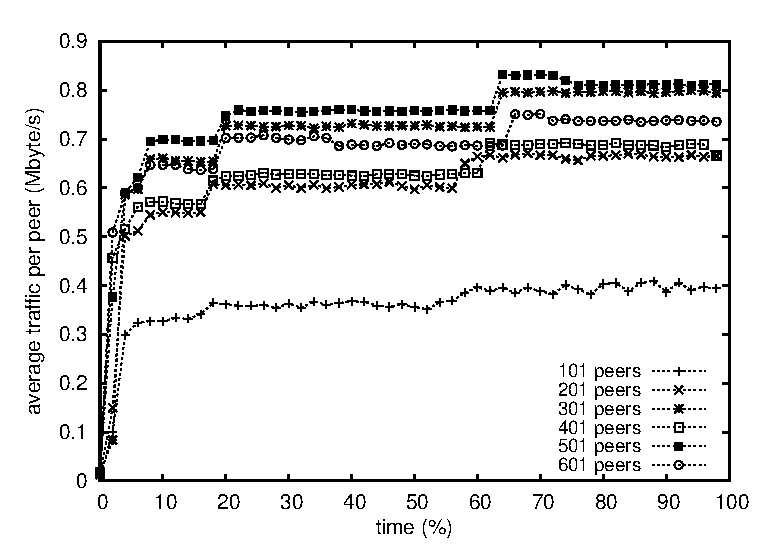
\includegraphics[width=0.8\textwidth]{img/traffic.eps}
  \caption{\label{fig:traffic} Traffic generated by editing sessions of
    various size.}
\end{figure}

%%% Local Variables: 
%%% mode: latex
%%% TeX-master: "../paper"
%%% End: 
